\documentclass[10pt,a4paper]{article}
\usepackage[utf8]{inputenc}
\usepackage{amsmath}
\usepackage{amsfonts}
\usepackage{amssymb}
\usepackage{graphicx}
\author{Brock Ellefson, Seth Severa}
\title{CSCI432 GW6}

\newcommand{\R}{\mathbb{R}}
\renewcommand{\thesubsection}{\thesection.\alph{subsection}}

\usepackage{algorithm}
\usepackage{algpseudocode}
\begin{document}
\maketitle
\section{Diversify your group}
We talked about this earlier, we will diversify for the next assignment.
\section{Recall the Skyline problem. Give pseudocode for the sweepline algorithm}
\section*{SkyLine sweep-line algorithm}
\begin{algorithm}
\caption{Skyline}\label{euclid}
\begin{algorithmic}[1]

\State List buildings
\State PriorityQueue events
\While {$currentBuilding \neq null$}
\State events.add(currentBuilding, currentBuilding.left)
\State events.add(currentBuilding, currentBuilding.right)
\State currentBuilding = currentBuilding.next
\EndWhile \\
\State List skyline
\State List currSkyline
\State double maxHeight = 0
\While {$events.peek()\neq null$}
\If{event.peek().isLeft()}
    \State currSkyline.add(event.peek())
    \If {$maxheight \neq checkMaxHeight(currSkyline)$}
    skyline.add(event.pop().left, checkmaxHeight(currSkyline))
    \EndIf
\Else
    \State currSkyline.remove(event.peek())
    \If {$maxheight \neq checkMaxHeight(currSkyline)$}
    skyline.add(event.pop().right, checkmaxHeight(currSkyline))
    \EndIf
\EndIf
\EndWhile
\State return skyline
\end{algorithmic}
\end{algorithm}
The loop invariant of this algorithm is that as the sweepline goes from left to right we always use the height of the current tallest building. 
\section{For the sweepline algorithm that computes whether there exist two line segments that intersect, explain how a line segment is added to or removed from T (the data structure that keeps track of the lines that intersect the sweep line).}
T is a red-black tree, we sweep through the graph from left to right, stopping at endpoints to check for intersections and add or remove line segments to T. Every time we stop at an endpoint, we check the order of T, if the order of T is different than the order of T from the previous endpoint we stopped at, then there was an intersection. After this check, if the endpoint of the line segment the sweepline is on is the leftmost endpoint of the line, then we add that line segment to the red-black tree. If the endpoint of the line segment the sweepline is on is the rightmost endpoint of the line, then we remove that line segment from the red-black tree.
\section{Union and Path Compression}
This is our beginning, a total of 8 components all of rank 0

	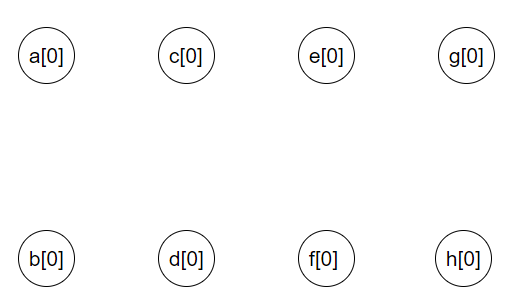
\includegraphics[scale = .5]{boi1.PNG}

This iteration combines two components of equal rank. Now a has a rank of one, and there are 7 components 

	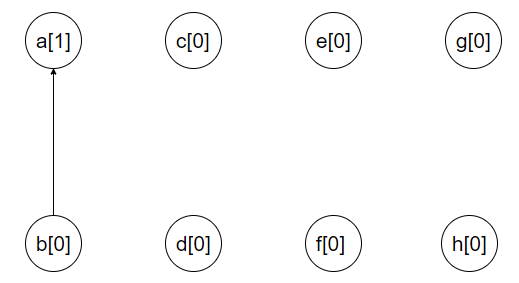
\includegraphics[scale = .5]{boi2.PNG}

This iteration combines two components of equal rank. Now a and c have a rank of one, and there are 6 components 

	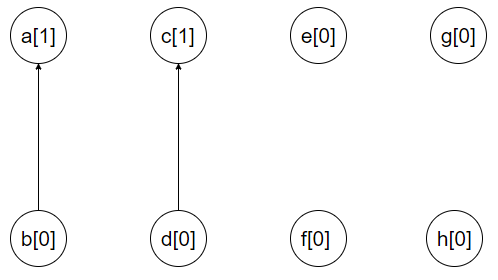
\includegraphics[scale = .5]{boi3.PNG}

This iteration adds the two components together, since a and c components both have the same rank, either could be the parent of the combined component, so we choose a. A's rank gets increased by 1, then we use path compression, and have d point to a as well. We know have 5 components.

	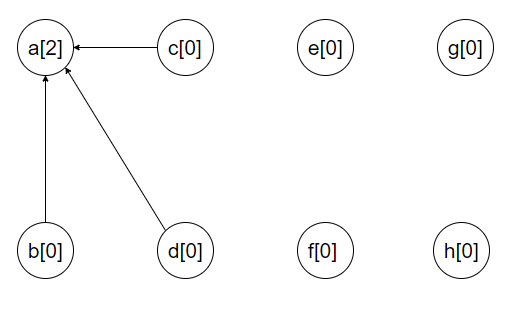
\includegraphics[scale = .5]{boi4.PNG}

This iteration combines two components of equal rank. Now e has a rank of one. We now have 4 components. 

	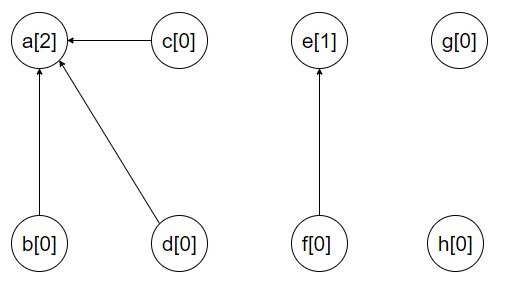
\includegraphics[scale = .5]{boi5.PNG}
	
This iteration combines two components of different rank. Since e has a higher rank than g, e will become g's parent. E's rank will not change. We know only have 3 components 

	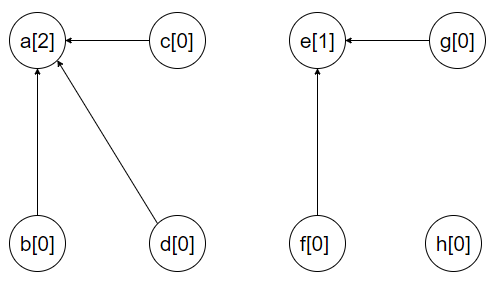
\includegraphics[scale = .5]{boi6.PNG}

\end{document}
